
\chapter{Vektor, Matrix, Tensor}



\section{Vektorraum}\label{vectorspace}
\index{Vektorraum}

Sei $(K,+,\cdot )$ ein Körper und $(V,+ ,\cdot)$ eine Menge mit zwei Verknüpfungen:
\begin{eqnarray*}
+ : V\times V &\longrightarrow& V \\
\cdot : K \times V &\longrightarrow& V 
\end{eqnarray*}
Hierbei ist zu beachten, dass die Verknüpfungen einmal auf $K$ und einmal auf $V$ definiert wurden. Man könnte hier verschiedene Zeichen zur Unterscheidung der Additionen einführen. Dies ist im allgemeinen aber unüblich, sodass hier vom Lernenden verlangt wird, den Unterschied selbst zu erkennen. Auf $V$ wird die Addition als \textsl{Vektoraddition} bezeichnet, sowie die Multiplikation als \textsl{Skalare Multiplikation}, da sie nicht zwischen zwei Vektoren, sondern einem Element des zugrunde liegenden Körpers und einem Vektor definiert ist. 

Man nennt $(V,+ ,\cdot)$ einen \textsl{Vektorraum}\index{Vektorraum} über dem Körper $K$, oder auch \textsl{K-Vektorraum}, wenn folgende Eigenschaften erfüllt sind:

\noindent Es seien $u,v,w \in V$ und $a,b \in K$:

Die Anforderungen an den Vektorraum werden in solche, die an die Addition (A*) und solche, die an die Multiplikation (M*) gestellt werden unterschieden:

\begin{description}
\item[(A1)] Assoziativgesetz: $u+(v+w) = (u+v)+w$
\item[(A2)] $0$ Element: $0\in V$ mit $v+0=0+v=v$
\item[(A3)] Inverses Element zur Addition: Zu jedem $v\in V$ gibt es ein $-v\in V$ mit $v+(-v) = -v+v = 0$
\item[(A4)] Kommutativgesetz: $u+v = v+u$
\end{description}

\begin{description}
\item[(M1)] Assoziativgesetz: $(a \cdot b)\cdot v = a\cdot (b\cdot v)$
\item[(M2)] 1 Element: $1\cdot v = v$
\item[(M3)] Distributivgesetz: $(a+b)\cdot v = a\cdot v + b\cdot v$
\item[(M4)] Distributivgesetz: $a\cdot(v+w) = a\cdot v + a\cdot w$
\end{description}

Es ist wichtig zu verstehen, wo die Unterschiede zwischen (M3) und (M4) liegen. (M3) besagt, dass die Summe zweier Zahlen in $K$ auf den Vektor $v$ verteilt (distribuiert) werden kann, während (M4) besagt, dass die Summe zweier Elemente aus $V$ auf $a$ verteilt werden kann. Das heißt: (M3) ist eine Eigenschaft der Addition in $K$ während (M4) eine Eigenschaft der Addition aus $V$ ist! 

\begin{svgraybox}
Zur Vertiefung der sei an dieser Stelle auf das grundlegende Werk von Egbert Brieskorn \cite{Brieskorn1} hingewiesen. 
\end{svgraybox}

\begin{definition}
Ein Element eines Vektorraums wird \textsl{Vektor} genannt.
\end{definition}

\subsection{Linearkombination}

\begin{definition}
Eine beliebige Summe von $p$ Vektoren $v_i \in V$ mit Faktoren $a_i \in K$ wird als \textsl{Linearkombination} bezeichnet.
\[
l = \sum_{i=1}^{p} a_i \cdot v_i = a_1\cdot v_1 + a_2 \cdot v_2 + \dots + a_p \cdot v_p
\]
Die Summe ist wiederum ein Vektor in $V$.

\end{definition}

\subsection{Basis}

Der Begriff der Basis ist an dieser Stelle noch nicht einführbar, ohne weitere Begriffe definiert zu haben, die aktuell von wenig Nutzen sind und den Lernenden eher verwirren. Daher beschränken wir uns aktuell nur auf eine Basis:

\begin{definition}
Als die \textsl{Standard-Basis} des $\mathbb{R}^n$ werden die Vektoren $e_i$ mit $i=1,\dots,n$ bezeichnet, deren Einträge überall null sind, bis auf den Eintrag $i$ und dieser ist 1. 
\begin{equation}
e_1 = \begin{pmatrix}
1\\
0\\
0\\
\vdots \\
0
\end{pmatrix}, e_2 = \begin{pmatrix}
0\\
1\\
0\\
\vdots \\
0
\end{pmatrix}, \dots, e_n = \begin{pmatrix}
0\\
0\\
\vdots \\
0\\
1
\end{pmatrix}
\end{equation}
\end{definition}

Jeder Vektor in $v\in V$ kann als Linearkombination dieser Basis geschrieben werden. Im Besonderen ist -- aufgrund der Wahl der Basisvektoren $e_i$ -- jeder Faktor dieser Linearkombination identisch mit dem $i$-ten Eintrag des Vektors. 

\[
v = \begin{pmatrix}
v_1 \\
v_2 \\
\vdots \\
v_n
\end{pmatrix} = \sum_{i=1}^{n} v_i \cdot e_i
\]

\subsection{Lineare Unabhängigkeit}

\begin{definition}
Die \textsl{linare Unabhängigkeit} \index{Unabhängigkeit, linear} von Vektoren wird definiert durch eine Linearkombination, d.h. eine Summe von Vektoren mit konstanten Faktoren. Wenn diese Linearkombination nur dadurch zu einem Null Vektor gemacht werden kann, indem alle Faktoren zu 0 werden, dann sind die Vektoren linear unabhängig. Seien $x_i$ aus einem K-Vektorraum und $\lambda_i $ aus dem zugrunde liegenden Körper. 

\begin{equation}\label{eq:linunabh}
\sum_{i=1}^{n} \lambda_i x_i = 0 \quad \text{dann, und nur dann, wenn} \quad \lambda_i = 0
\end{equation}
\end{definition}

Dies sollte näher erklärt werden: Nehmen wir ein einfaches Beispiel und sehen uns zwei Vektoren in der Ebene an. 

\bigskip

\begin{center}
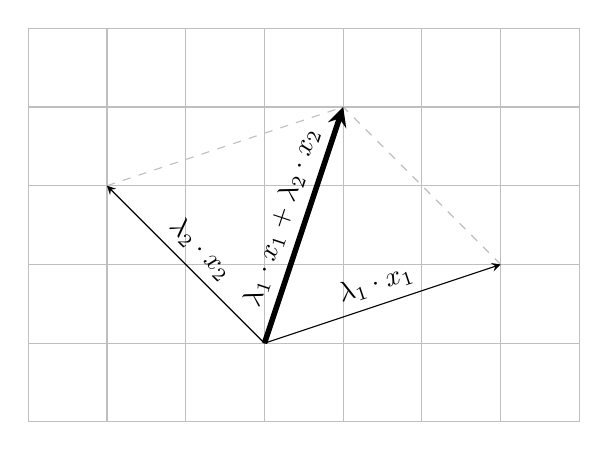
\begin{tikzpicture}[>=stealth]
\coordinate (A) at (0,0);
\coordinate (B) at (3,1);
\coordinate (C) at (1,3);
\coordinate (D) at (-2,2);
\tikzset{-}
\draw[lightgray, step=1cm] (-3,-1) grid (4,4);
\tikzset{-}
\draw[lightgray, dashed] (D) -- (C);
\draw[lightgray, dashed] (B) -- (C);
\tikzset{->}
\draw (A) -- (B) node[midway, sloped, above] {$\lambda_1 \cdot x_1$};
\draw (A) -- (D) node[midway, sloped, above] {$\lambda_2 \cdot x_2$};
\draw[line width=2] (A) -- (C) node[midway, sloped, above] {$\lambda_1 \cdot x_1+\lambda_2 \cdot x_2$};
\end{tikzpicture}
\end{center}

\bigskip

Per Definition der linearen Unabhängigkeit kann der dicke Pfeil nur dann die Länge 0 haben, wenn $\lambda_1$ und $\lambda_2$ beide 0 sind. Salopp gesprochen könnte man sagen: Der Durchmesser eines Parallelograms\footnote{Ein Viereck dessen gegenüberliegenden Seiten parallel zueinander sind, nennt man Parallelogramm.} -- wie das, welches die Vektoren aufspannen -- kann nur dann 0 sein, wenn die Seitenlängen 0 sind.

\subsection{Dimension}

\begin{definition}
Die maximale Anzahl von linear unabhängigen Basisvektoren eines Vektorraums wird \textsl{Dimension}\index{Dimension} genannt. Der $\mathbb{R}^n$ hat die Dimension $n$, da es genau $n$ Möglichkeiten gibt, Basisvektoren zu bilden, die aus $n-1$ Nullen und einer 1 bestehen.
\end{definition}


\section{Lineare Gleichungssysteme}

Lineare Gleichungssysteme treten häufig in der Physik und den Ingenieurswissenschaften auf. Dabei handelt es sich um Probleme in mehreren Unbekannten, die durch eine Reihe von Randbedingungen -- in Form von Gleichungen -- spezifiziert werden.

Bei diesen Problemen ist es notwendig, dass alle Unbekannte die Randbedingungen gleichzeitig erfüllen:

\begin{equation}\label{eq:syseq}
\begin{split}
a_{1,1}x_1 + a_{1,2}x_2 + \dots + a_{1,n}x_n &= b_1 \\
a_{2,1}x_1 + a_{2,2}x_2 + \dots + a_{2,n}x_n &= b_2 \\
a_{3,1}x_1 + a_{3,2}x_2 + \dots + a_{3,n}x_n &= b_3 \\
\vdots &= \vdots \\
a_{m,1}x_1 + a_{m,2}x_2 + \dots + a_{m,n}x_n &= b_m 
\end{split}
\end{equation}
Die Werte für $a_{i,j}$ und $b_{i}$ sind vorgegeben. Gesucht werden die $x_j$ Werte. 

Gleichungssysteme werden nach der Anzahl ihrer Gleichungen in folgende Kategorien eingeteilt:

\begin{description}
\item[$m<n$] Solche Systeme bezeichnet man als \textsl{unterbestimmt}, es existieren weniger Gleichungen als Unbekannte. Die Lösung solcher Systeme ist im allgemeinen nicht eindeutig. Solche Gleichungssysteme treten in der linearen Optimierung auf. 
\item[$m>n$] Solche Systeme bezeichnet man als \textsl{überbestimmt}, es existieren mehr Gleichungen als Unbekannte. Es ist im allgemeinen nicht möglich eine Lösung für solche Systeme anzugeben, da es möglich ist, sich widersprechende Randbedingungen in den Gleichungen zu formulieren. 
\item[$m=n$] Auch als quadratische Gleichungssysteme bezeichnet. Sofern bestimmte Bedingungen von den $a_{i,j}$ Werten erfüllt werden, gibt es genau eine Lösung. Dies sind die Systeme, mit denen wir uns hier beschäftigen werden.
\end{description}

\subsection{Kompakte Notation}

Mathematiker machen sich gerne das Leben einfacher, in dem sie ihre Formeln abkürzen. Das Gleichungssystem (\ref{eq:syseq}) ist sehr unhandlich. Daher führen wir folgende Schreibweisen ein:

Wir schreiben die $x_j$ und $b_i$ Werte in einer Spaltenform: 

\[
x = \begin{pmatrix}
x_1 \\
x_2 \\
\vdots \\
x_n
\end{pmatrix}, \quad b = \begin{pmatrix}
b_1 \\
b_2 \\
\vdots \\
b_m
\end{pmatrix}
\]
Sowie für die $a_{i,j}$ Werte eine rechteckige Tabellenform:

\[
A = \begin{pmatrix}
a_{1,1} & a_{1,2} & \cdots & a_{1,n} \\
a_{2,1} & a_{2,2} & \cdots & a_{2,n} \\
\vdots & \vdots & \ddots & \vdots \\
a_{m,1} & a_{m,2} & \cdots & a_{m,n}
\end{pmatrix}
\]

Definieren wir nun eine Multiplikation zwischen der rechteckigen Tabellenform und einer Spaltenform auf diese Weise:
\begin{equation*}
a_{i,1}x_1 + a_{i,2}x_2 + \dots + a_{1,n}x_n = \sum_{j=1}^{n} a_{i,j}x_j
\end{equation*}
für jede Zeile $i$, so lässt sich das Gleichungssystem (\ref{eq:syseq}) schreiben als:

\begin{equation*}
\begin{pmatrix}
a_{1,1} & a_{1,2} & \cdots & a_{1,n} \\
a_{2,1} & a_{2,2} & \cdots & a_{2,n} \\
\vdots & \vdots & \ddots & \vdots \\
a_{m,1} & a_{m,2} & \cdots & a_{m,n}
\end{pmatrix} \cdot \begin{pmatrix}
x_1 \\
x_2 \\
\vdots \\
x_n
\end{pmatrix} = \begin{pmatrix}
b_1 \\
b_2 \\
\vdots \\
b_m
\end{pmatrix}
\end{equation*}
oder
\begin{equation*}
Ax=b
\end{equation*}

Hier haben wir uns noch keine Gedanken darüber gemacht, was diese Spalten und Tabellen eigentlich sind. Sie stellen für uns lediglich eine Vereinfachung der Schreibweise dar. Später werden wir erkennen, dass die Spalten Vektoren sind und die Tabelle eine Matrix.


\subsection{Matrix}

\begin{definition}
Eine \textsl{Matrix} \index{Matrix} ist eine rechteckige Struktur von Elementen des Körpers, über dem sie gebildet werden. Hier werden im allgemeinen nur reelle Matrizen betrachtet. Somit sind diese Matrizen aus dem $\mathbb{R}^{m\times n}$:
\end{definition}

\begin{equation*}
(A)_{i,j} = a_{i,j} \in \mathbb{R}
\end{equation*}

Mit der Matrix Addition und der Skalaren Multiplikation
\begin{eqnarray*}
A+B &=& (a_{i,j} + b_{i,j})_{i,j} \\
\alpha A &=& (\alpha a_{i,j})_{i,j}
\end{eqnarray*}
wird der $\mathbb{R}^{m\times n}$ zu einem Vektorraum. Das Nachrechnen der A1-A4 und M1-M4 Eigenschaften aus Kapitel \ref{vectorspace} ist Teil der Aufgaben.

Dabei ist zu beachten, dass $0 \in \mathbb{R}^{m\times n} = (0)_{i,j}$ die Null Matrix ist, und das neutrale Element der Multiplikation die Einsmatrix $\mathbf{1}$, oder auch Identität $I$ genannt:

\[
\mathbf{1} = I =
\begin{pmatrix}
1 & 0 & 0 & \cdots & 0 \\
0 & 1 & 0 & \cdots & 0 \\
0 & 0 & 1 & \cdots & 0 \\
\vdots & \vdots & \vdots & \ddots & \vdots \\
0 & 0 & 0 & \cdots & 1
\end{pmatrix}
\]

\subsubsection{Rechenregeln}

\begin{definition}
Die Zahlen in den einzelnen Zellen der Tabelle nennt man \textsl{Einträge} oder auch \textsl{Komponenten}. Das selbe gilt für einen Vektor, der als einspaltige Matrix interpretiert werden kann.
\end{definition}

Die Addition zweier Matrizen wird auf die einzelnen Einträge abgebildet. Als Abkürzung wird hier die Notation $(\dots)_{i,j}$ verwendet. Dies ist eine Darstellung des Eintrags an der $i$-ten Zeile und $j$-ten Spalte. Wenn keine Einschränkung an $i$ und $j$ gemacht werden, so gilt diese Abkürzung für jeden Eintrag der Matrix. Und somit bestimmt diese Abkürzung auch die gesamte Matrix.

\begin{equation*}
A + B = \left( a_{i,j} + b_{i,j} \right)_{i,j} = \begin{pmatrix}
a_{1,1}+b_{1,1} & a_{1,2}+b_{1,2} & \cdots & a_{1,n}+b_{1,n} \\
a_{2,1}+b_{2,1} & a_{2,2}+b_{2,2} & \cdots & a_{2,n}+b_{2,n} \\
\vdots & \vdots & \ddots & \vdots \\
a_{m,1}+b_{m,1} & a_{m,2}+b_{m,2} & \cdots & a_{m,n}+b_{m,n}
\end{pmatrix}
\end{equation*}
In gleicher Weise wird die skalare Multiplikation realisiert

\begin{equation*}
\alpha \cdot A = \left( \alpha \cdot a_{i,j} \right)_{i,j} = \begin{pmatrix}
\alpha \cdot a_{1,1} & \alpha \cdot a_{1,2} & \cdots & \alpha \cdot a_{1,n} \\
\alpha \cdot a_{2,1} & \alpha \cdot a_{2,2} & \cdots & \alpha \cdot a_{2,n} \\
\vdots & \vdots & \ddots & \vdots \\
\alpha \cdot a_{m,1} & \alpha \cdot a_{m,2} & \cdots & \alpha \cdot a_{m,n}
\end{pmatrix}
\end{equation*}

Die Multiplikation von Matrizen $A,B$ ist in der Form definiert, dass der Eintrag an der Stelle $i,j$ definiert ist durch die Summe der Produkte der Einträge der $i$-ten Zeile von A mit den Einträgen der $j$-ten Spalte von B. Sei $A\in \mathbb{R}^{m\times n}$ und $B\in \mathbb{R}^{n\times o}$

\begin{equation*}
\begin{split}
A \cdot B & = \left( \sum_{k=1}^{n} a_{i,k} \cdot b_{k,j} \right)_{i,j} \\
 &= \begin{pmatrix}
\left( \sum_{k=1}^{n} a_{1,k} \cdot b_{k,1} \right) & \left( \sum_{k=1}^{n} a_{1,k} \cdot b_{k,2} \right) & \cdots & \left( \sum_{k=1}^{n} a_{1,k} \cdot b_{k,o} \right) \\
\left( \sum_{k=1}^{n} a_{2,k} \cdot b_{k,1} \right) & \left( \sum_{k=1}^{n} a_{2,k} \cdot b_{k,2} \right) & \cdots & \left( \sum_{k=1}^{n} a_{2,k} \cdot b_{k,o} \right) \\
\vdots & \vdots & \ddots & \vdots \\
\left( \sum_{k=1}^{n} a_{m,k} \cdot b_{k,1} \right) & \left( \sum_{k=1}^{n} a_{m,k} \cdot b_{k,2} \right) & \cdots & \left( \sum_{k=1}^{n} a_{m,k} \cdot b_{k,o} \right) \\
\end{pmatrix}
\end{split}
\end{equation*}

Aus dieser Definition folgt, dass die Anzahl der Spalten der Matrizen links vom Multiplikationszeichen und die Anzahl der Zeilen der Matrix rechts vom Multiplikationszeichen identisch sein müssen. Sind sie nicht identisch, ist die Mulitplikation \textbf{nicht} definiert und die Matrizen können nicht miteinander multipliziert werden. Des Weiteren besitzt die resultierende Matrix soviel Zeilen, wie Matrix $A$ aber soviel Spalten wie Matrix $B$.

\begin{svgraybox}
Hat Matrix $B$ nur eine Spalte ($B\in \mathbb{R}^{n\times 1}$) -- ist also ein Vektor --, dann ist dadurch auch gleichzeitig die Matrix-Vektor Multiplikation definiert. 
\end{svgraybox}

Seien $A\in \mathbb{R}^{m\times n}$ und $b\in \mathbb{R}^{n\times 1}$, dann ist die Matrix-Vektor Multiplikation

\begin{equation*}
A \cdot b = \left( \sum_{k=1}^{n} a_{i,k} \cdot b_{k} \right)_{i} = \begin{pmatrix}
\left( \sum_{k=1}^{n} a_{1,k} \cdot b_{k} \right) \\
\left( \sum_{k=1}^{n} a_{2,k} \cdot b_{k} \right) \\
\vdots \\
\left( \sum_{k=1}^{n} a_{m,k} \cdot b_{k} \right) \\
\end{pmatrix}
\end{equation*}
Im Weiteren ist der $\mathbb{R}^{n\times 1} = \mathbb{R}^n$.


\subsubsection{Transposition}

Die Transponierte einer Matrix erhält man durch vertauschen der Indizes. Sei $A \in \mathbb{R}^{m\times n} $ eine Matrix. 

\begin{definition}
Die Transponierte $A^T \in \mathbb{R}^{n\times m}$ ist definiert durch:
\[
	A^T = (a_{j,i})_{i=1,\dots, n; j=1,\dots, m}
\]
\end{definition}
Das Transponieren gilt auch für Vektoren genauso, da diese ja einspaltige Matrizen sind. Sei $v\in \mathbb{R}^{m\times 1}$ ein Vektor. Der transponierte Vektor $v^T$ ist dann im aus dem Raum $\mathbb{R}^{1\times m}$

\[
v^T = \begin{pmatrix}
v_1\\
v_2\\
\vdots \\
v_m
\end{pmatrix}^T = (v_1, v_2, \dots , v_n)
\]

Aufgrund der Regel, dass Matrizen nur dann miteinander multipliziert werden dürfen, wenn die Spalten-Anzahl der linken Matrix mit der Zeilen-Anzahl der rechten Matrix übereinstimmen muss, konnten Vektoren bisher nicht an Matrizen von links multipliziert werden. Mit dem transponierten Vektor geht dies, da er eine Spalten-Anzahl hat, die mit der Matrix übereinstimmen kann. Seien wieder $v\in \mathbb{R}^m$ und $A\in \mathbb{R}^{m\times n}$.

\[
v^T \cdot A = (\sum_{i=1}^{m}v_i\cdot a_{i,j})_{j} = \begin{pmatrix}
\sum_{i=1}^{m}v_i\cdot a_{i,1} \\
\sum_{i=1}^{m}v_i\cdot a_{i,2} \\
\vdots \\
\sum_{i=1}^{m}v_i\cdot a_{i,n}
\end{pmatrix} \in \mathbb{R}^n
\]

\subsubsection{Rang und Determinante}

TODO

\section{Algebraische Strukturen}

TODO

\subsection{Eigenschaften von Abbildungen}


\begin{definition}
Eine Abbildung $\phi : V \longrightarrow W$ wird als \textsl{injektiv}\index{injektiv} bezeichnet, wenn für $u,v \in V$ 
\[ u\ne v \Rightarrow \phi(u) \ne \phi(v) \]
\end{definition}
Umgekehrt gilt: Aus $\phi(u)=\phi(v)$ folgt, dass $u=v$ ist. 

\begin{definition}
Eine Abbildung $\phi : V \longrightarrow W$ wird als \textsl{surjektiv}\index{surjektiv} bezeichnet, wenn für alle $w\in W$ mindestens ein $v\in V$ existiert mit 
\[\phi(v) = w\]
\end{definition}

\begin{definition}
Eine Abbildung $\phi : V \longrightarrow W$ wird als \textsl{bijektiv}\index{bijektiv} bezeichnet, wenn sie sowohl injektiv als auch surjektiv ist. 
\end{definition}

Aufgrund der Surjektivität gibt es zu $w\in W$ immer ein $v\in V$  mit $\phi(v)=w$ und dieses $v$ ist eindeutig aufgrund der Injektivität. Daher gilt eine bijektive Abbildung $\phi$ als \textsl{umkehrbar eindeutig}\index{umkehrbar eindeutig}. D.h. es gibt ein $\phi^{-1} : W \longrightarrow V$ mit $v = \phi^{-1}(w)$.

\subsection{Morphologie}

\begin{definition}

Ein \textsl{Vektorraumhomomorphismus}\index{Homomorphismus}\index{Vektorraumhomomorphismus} -- auch verkürzt einfach Homomorphismus genannt -- von $V$ nach $W$ ist eine Abbildung $\phi : V \longrightarrow W$ mit folgenden Eigenschaften:
\begin{enumerate}
\item Für alle $v,w \in V$ gilt: $\phi(v+w) = \phi(v)+\phi(w)$
\item Für alle $a\in K$ und $v\in V$ ist $\phi(av)=a\phi(v)$
\end{enumerate}
Ist $V=W$, so wird $\phi : V\longrightarrow V$ als \textsl{Endomorphismus}\index{Endomorphismus} bezeichnet.
\end{definition}

\begin{definition}
Ist $\phi : V\longrightarrow W$ ein bijektiver Homomorphismus, so wird $\phi$ als \textsl{Isomorphismus}\index{Isomorphismus} bezeichnet.
\end{definition}

\begin{definition}
Ist $\phi : V\longrightarrow V$ ein bijektiver Endomorphismus,  so wird $\phi$ als \textsl{Automorphismus}\index{Automorphismus} bezeichnet.
\end{definition}

\subsection{Linearformen}

\begin{definition}
Eine \textsl{Linearform} \index{Linearform} ist eine lineare Abbildung von einem K-Vektorraum in seinen zugrundeliegenden Körper
\[
l : V \longrightarrow K
\]
mit der Eigenschaft
\[l(\alpha v + \beta w) = \alpha l(v) + \beta l(w) \]
für $v,w\in V$ und $\alpha, \beta \in K$
\end{definition}

\subsubsection{Bilinearformen}

\begin{definition}
Seien $V,W$ K-Vektorräume. Eine \textsl{Bilinearform} $b$ ist eine lineare Funktion
\[
	b : V \times W \longrightarrow K
\]
mit den Eigenschaften:
\begin{eqnarray*}
b(\alpha v + \beta w,x) &=& \alpha b(v,x) + \beta b(w,x) \\
b(v,\alpha w + \beta x) &=& \alpha b(v,w) + \beta b(v,x) 
\end{eqnarray*}
für $v\in V$, $w\in W$ und $\alpha, \beta \in K$. Um genau zu sein ist eine Bilinearform eine zwei Parametrige lineare Funktion, die sich in beiden Parametern wie eine Linearform verhält.
\end{definition}

Jede Bilinearform hat eine Matrix-Darstellung, denn zu jeder Bilinearform $\beta(.,.)$ kann folgende Matrix definiert werden:
\[
B = (b_{i,j})_{i,j} := (\beta(e_i, e'_j))_{i,j}
\]
mit den Basisvektoren $e_i\in V$ und $e'_j\in W$.

\begin{definition}
Eine spezielle Bilinearform $\langle .,.\rangle : V\times V \longrightarrow K$ wird \textsl{Skalarprodukt} oder auch \textsl{inneres Produkt} genannt. (Man darf dies nicht mit der Skalarmultiplikation verwechseln, also dem Produkt aus einer Zahl aus dem Körper mit einem Vektor). In reellen Vektorräumen nimmt es die folgende Form an:
\[
\langle u,v \rangle = \sum_{i=1}^{n} u_i\cdot v_i = u^T \cdot v
\]
für $u,v \in V$
\end{definition}

\begin{definition}
Seien $u,v \in V$ und $\langle .,.\rangle$ ein Skalarprodukt auf $V$. Seien $u\ne 0$ und $v\ne 0$. Falls 
\[ \langle u,v \rangle = \langle v,u \rangle = 0\]
ist, so bezeichnet man $u$ und $v$ als zueinander \textsl{orthogonal}. \index{orthogonal}
\end{definition}


\subsubsection{Definitheit}


\begin{definition}
Sei $b(.,.)$ eine Bilinearform. $b(.,.)$ ist

\begin{enumerate}
\item \textsl{positiv definit}, falls $b(v,v)>0$\index{positiv definit}
\item \textsl{positiv semidefinit}, falls $b(v,v)\ge 0$\index{positiv semidefinit}
\item \textsl{negativ definit}, falls $b(v,v) <0$\index{negativ definit}
\item \textsl{negativ semidefinit}, falls $b(v,v)\le 0$\index{negativ semidefinit}
\end{enumerate}
für alle $v\in V $
\end{definition}



\subsubsection{Norm und Abstände}

\begin{definition}
Eine \textsl{Norm}\index{Norm} ist eine lineare Abbildung $\Vert . \Vert : V \longrightarrow \mathbb{R}_+$, vom Vektorraum in die positiven reellen Zahlen. Dabei gelten folgende Eigenschaften:
\begin{description}
\item[(1)] Aus $\Vert v\Vert = 0$ folgt $v=0$
\item[(2)] $\Vert a\cdot v\Vert = \vert a\vert \cdot \Vert v\Vert$
\item[(3)] $\Vert u+v\Vert \le \Vert u\Vert + \Vert v\Vert $ (Dreiecksungleichung)
\end{description}
Mit $u,v\in V$, $a\in K$ und $\vert a\vert$ dem Absolutbetrag des Skalars $a$.
\end{definition}
Zu beachten ist, dass die Norm nicht in den zugrundeliegenden Körper abbildet. Falls $K=\mathbb{C}$, dann ist trotzdem das Ergebnis der Norm in den positiven reellen Zahlen. Ein Vektorraum, in dem eine Norm definiert ist, nennt man einen \textsl{normierten Raum}\index{Raum, normiert}, oder \textsl{normierter Vektorraum}.

\begin{definition}
Sei $V$ ein reeller Vektorraum $\mathbb{R}^n$ mit einem Skalarprodukt $\langle .,.\rangle$. Die Linearform 
\[
\Vert u \Vert = \sqrt{\langle u,u \rangle}
\]
wird \textsl{euklidische Norm}\index{Norm, euklidische} oder vom Skalarprodukt \textsl{induzierte Norm}\index{Norm, induziert} genannt. Sie ist hier separat definiert, da sie in diesem Kapitel eine zentrale Rolle spielt. Die folgenden Definitionen sind ebenfalls korrekt:
\begin{equation}\label{eq:2norm}
\Vert u \Vert = \sqrt{u^T \cdot u} = \sqrt{\sum_{i=1}^{n} u_i^2}= \sqrt{\sum_{i=1}^{n} \vert u_i \vert^2}
\end{equation}
\end{definition}

Dass die Euklidische Norm die Eigenschaften (1)-(3) erfüllt, soll in den Aufgaben nachgerechnet werden. Normen stellen ein wichtiges Werkzeug dar, denn mit ihnen können Längen von Vektoren gemessen werden. Einen Vektorraum, in dem ein Skalarprodukt definiert ist, nennt man einen \textsl{Skalarproduktraum}.\index{Skalarproduktraum}\index{Raum mit Skalarprodukt}

\begin{definition}
Eine Bilinearform $d : V\times V \longrightarrow \mathbb{R}_+$ heißt \textsl{Metrik}\index{Metrik}, falls folgende Eigenschaften erfüllt sind:
\begin{description}
\item[(1)] Aus $d(u,v) = 0$ folgt $u=v$
\item[(2)] $d(u,v) = d(v,u)$, diese Eigenschaft wird auch als Symmetrie bezeichnet.
\item[(3)] $d(u,w) \le d(u,v) + d(u,w)$ (Dreiecksungleichung)
\end{description}
\end{definition}

Eine Metrik wird dazu benutzt einen Abstand zwischen zwei Vektoren zu messen. Ein Vektorraum, in dem eine Metrik definiert ist, nennt man \textsl{metrischen Raum}\index{Raum, metrisch}. 

\begin{definition}
Jeder normierte Raum kann zu einem metrischen Raum gemacht werden, indem eine Metrik auf Basis der Norm definiert wird:
\[
d(u,v) = \Vert u-v \Vert
\]
\end{definition}

\begin{definition}
In Anlehnung an Formel (\ref{eq:2norm}) kann allgemein eine \textsl{p-Norm} definiert werden:
\[
\Vert u \Vert_p = \left( \sum_{i=1}^{n} \vert u_i \vert^p \right)^{\frac{1}{p}}
\]
für $p\in \mathbb{N}$. Nach dieser Definition ist die euklidische Norm eine 2-Norm. 
\end{definition}

Für $p \longrightarrow \infty$ nähert sich die Norm immer weiter an den größten Wert der $\vert u_i \vert$ an, da dieser mit dem immer größer werdenden Exponenten die Summe immer weiter beherrscht. Es gilt also für $p=\infty$
\[
\Vert u \Vert_\infty = \max_{i=1,\dots, n}  \vert u_i\vert
\]
(Der Beweis, dass die $\infty -Norm$ gleich dem absoluten Maximum ist, wird nachgeliefert. Dafür ist eine Grenzwertbetrachtung notwendig, die bisher noch nicht erklärt wurde).

\subsection{Dualraum}

\begin{definition}
Die Menge aller Linearformen eines K-Vektorraums werden \textsl{Dualraum} von V genannt. Der Dualraum wird meist mit einem Stern gekennzeichnet
\[V^* \]
\end{definition}

Aufgrund der Eigenschaften der Linearformen bilden diese einen eigenen Vektorraum. 

\subsection{Skalarproduktraum}

\begin{definition}
Ein \textsl{Skalarproduktraum} ist ein K-Vektorraum $(V,+,\cdot)$ zusammen mit einem Skalarprodukt $\langle .,. \rangle$.
\end{definition}

Jeder Skalarproduktraum wird mit 
\[ \Vert u \Vert = \sqrt{\langle u,u \rangle} \]
zu einem normierten Raum \index{Raum, normiert}. Sowie mit 
\[ d(u,v) = \Vert u-v \Vert \]
zu einem metrischen Raum. \index{Raum, metrisch} In diesem Sinne ist die Definition eines Skalarproduktes die erste Wahl zur Erweiterung eines Vektorraums. 



\section{Tensor}

TODO

\section{Aufgaben}

\begin{prob}
\label{matrix.1}

Weise nach, dass der $\mathbb{R}^{m\times n}$ ein Vektorraum ist. 

\end{prob}


